\documentclass[tikz]{standalone}
\usepackage{tikz}
\usetikzlibrary{arrows}
\usetikzlibrary{scopes}
\usepackage{xcolor}
\begin{document}
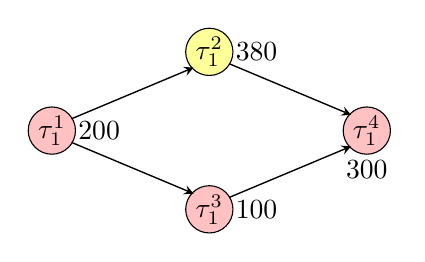
\begin{tikzpicture}


%\definecolor{lgray}{RGB}{127,130,183};
%
%\definecolor{lgb}{RGB}{96,173,193};
%RED
%{250,1288,114}
%{255,69,0}
%{250,164,96}
%{255,160,122}
%{254,125,139}
%{255,193,194}

%YELLOW
%{222,170,34}
%{255,230,0}

\definecolor{tomato}{RGB}{255,193,194};
\definecolor{gold}{RGB}{254,255,153};

%\definecolor{dred}{RGB}{176,0,0}
%\definecolor{violet}{RGB}{238,130,238};
%\definecolor{cyan}{RGB}{0,255,255};

\draw [fill=white,draw=white] (0,0) rectangle (0,0.1);

%draw rectangles

%\draw [fill=lgb,draw=black] (1,4) rectangle (2,5);
%	
%\draw [fill=lgb,draw=black] (3,4) rectangle (4,5);
%	
%\draw [fill=lgb,draw=black] (5,4) rectangle (6,5);
%	
%\draw [fill=lgb,draw=black] (7,4) rectangle (8,5);
%\draw [fill=lgb,draw=black] (9,4) rectangle (10,5);
%
%		
%
%
%\draw [fill=lgray,draw=black] (0,2) rectangle (2,3);
%\draw [fill=lgray,draw=black] (3,2) rectangle (5,3);
%\draw [fill=lgray,draw=black] (6,2) rectangle (8,3);
%\draw [fill=lgray,draw=black] (9,2) rectangle (11,3);
	
	
%\draw [fill=lgry,draw=black] (1,0) rectangle (4,1);
%\draw [fill=lgry,draw=black] (5,0) rectangle (6,1);
%\draw [fill=lgry,draw=black] (7,0) rectangle (10,1);

%	
%	
%	\filldraw [fill=gray,draw=black] (2,0) rectangle (3,0.7);
%	\filldraw [fill=black,draw=black] (1.5,0) rectangle (2,0.7);
%	\filldraw [fill=gray,draw=black] (5,0) rectangle (6.5,0.7);
%	\filldraw [fill=gray,draw=black] (8,0) rectangle (9.5,0.7);
	

	{[fill=tomato,draw=black]
			
		\filldraw (0,1) circle (0.3cm);
		\node at (0,1) {\textcolor{black}{$\tau_1^1$}};
		\node at (0.6,1) {\textcolor{black}{$200$}};
		
		\filldraw (2,0) circle (0.3cm);
		\node at (2,0) {\textcolor{black}{$\tau_1^3$}};
		\node at (2.6,0) {\textcolor{black}{$100$}};
		
		\filldraw (4,1) circle (0.3cm);
		\node at (4,1) {\textcolor{black}{$\tau_1^4$}};
		\node at (4,0.5) {\textcolor{black}{$300$}};
		
}
	
	{[fill=gold,draw=black]
		
		\filldraw (2,2) circle (0.3cm);
		\node at (2,2) {\textcolor{black}{$\tau_1^2$}};
		\node at (2.6,2) {\textcolor{black}{$380$}};
		}
	
	{[->,>=stealth,line width=0.5pt]
		% from $v_0$
	 \draw (0.25,1.15)--(1.8,1.8);
	 \draw (0.25,0.85)--(1.8,0.2);
	 
	 \draw (2.25,1.85)--(3.8,1.2);
	 \draw (2.25,0.15)--(3.8,0.8);

%	 
	
%	 
	
	  
	   
	   
	   
	   % from $v_1$
	   
	   
	 }
	
	
%\draw[->,>=triangle 45,line width=1.5pt,color=red] (13,1)--(11,0.5);
%\node [below, color=red] at(12.5,1.6) {\large miss deadline};

%	\foreach \x in {0,4,8,12}
%	\draw [->,>=triangle 45,line width=2pt] (\x,0)--(\x,1.5);
%	\foreach \x in {3,7,11}
%	\draw [->,>=triangle 45,line width=2pt] (\x,1.5)--(\x,0);
%	
%
%
%%draw time line
%\draw[->,>=triangle 45,line width=2pt] (-1,0)--(13,0);
%\node [below] at (13,0) {\Large time};
%
%{[dashed,line width=1pt]
%	\foreach \x in {0,3}
%	\draw[] (\x,0)--(\x,2.5);
%	\draw[](4,0)--(4,2.5);
%	\draw[](8,0)--(8,2.5);
%	\draw[](12,0)--(12,2.5);
%	\draw[](2,1)--(2,-1);
%	\draw[](9.5,1)--(9.5,-1);
%}
%
%
%\draw[<->,>=triangle 45, line width=1.5pt] (2,-0.5)--(9.5,-0.5);
%\node [rectangle,fill=black] at (5.5,-0.5) {\Large{$L_k$}};
%\foreach \x in {0,4,8}
%\draw[<->,>=triangle 45,line width=1.5pt] (\x,2.5)--(\x+4,2.5);
%\foreach \x in {2,6,10}
%\node [rectangle,fill=black] at (\x,2.5) {\Large{$T_i$}};
%
%\draw[<->,>=triangle 45,line width=1.5pt] (0,2)--(3,2);
%\node [rectangle,fill=black] at (1.5,2) {\Large{$R_i$}};
%
%{[->,>=triangle 45,dashed,line width=1pt, color=red]
%	\draw[](0.5,-0.25)--(2.5,0.3);
%	\node [] at (0.5,-0.5) {\Large{carry-in job}};
%	\draw[](5.5,1.25)--(6,0.3);
%	\node [] at (5.5,1.4) {\Large{body job}};
%	\draw[](9.5,1.25)--(9,0.3);
%	\node [] at (9.5,1.4) {\Large{carry-out job}};
%	
%	}
%
%\node [below] at (2,0) {\Large{$t_0$}};
%\node [below] at (9.5,0) {\Large{$f_k$}};
%
%\filldraw [fill=black,draw=black] (12.5,0.2) rectangle (15.3,4.5);
%\draw [->,>=triangle 45,line width=2pt] (13,2.5)--(13,4);
%\node [below] at (14,3.5) {\Large{Release}};
%
%\draw [<-,>=triangle 45,line width=2pt] (13,0.5)--(13,2);
%\node [below] at (14.3,1.5) {\Large{Deadline}};

\end{tikzpicture}
\end{document}
